\documentclass[12pt]{article}

\usepackage[utf8]{inputenc}
\usepackage[T1]{fontenc}
\usepackage{a4}
\usepackage{lipsum}
\usepackage{graphicx}
\usepackage{float}
\usepackage{listings}
\usepackage{color}
\usepackage{hyperref}
\usepackage{cite}
\usepackage{textgreek}
\usepackage{amsfonts}
\usepackage{amsmath}

\usepackage[margin=1in]{geometry}

\title{
  {\Huge \bf Power Systems Lab}\\
  \vspace{0.25in}

  {\bf Experiment 10}\\
  Laboratory Report
  \vspace{1in}
}
\author{
  \bf Syed Alisamar Husain, 17BEE012\\
  B.Tech Electrical Engg, 8th Semester
}

\begin{document}
  \begin{titlepage}
    \maketitle
    \vspace*{\fill}
    \begin{center}
      {\bfseries Department of Electrical Engineering} \\
      Jamia Millia Islamia, New Delhi
    \end{center}
    \thispagestyle{empty}
  \end{titlepage}
  
  \newpage
  \begin{center}
    \huge Experiment 10
    \vspace{0.5in}
  \end{center}

  \section{Objective}
  Develop a Simulink model for a series compensated 
  transmission line.

  \section{Theoretical Background}
  Series compensation is the method of improving the system 
  voltage by connecting a capacitor in series with the transmission line. 
  In other words, in series compensation, reactive power is inserted in 
  series with the transmission line for improving the impedance of the system. 
  
  It improves the power transfer capability of the line. It is mostly 
  used in extra and ultra high voltage line.

    \subsection{Advantages of Series Compensation}
    Series compensation has several advantages like it increases transmission 
    capacity, improve system stability, control voltage regulation and ensure 
    proper load division among parallel feeders.

    \begin{itemize}
      \item {\bf Increase in Power Transfer Capability}\\ The power transfer over a line is given by
      \begin{center}
        $ P_1 = \dfrac{V_S V_R}{X_L} sin \delta $
      \end{center}
      If a capacitor having capacitance reactance $X_C$ is connected in series with the line, 
      the reactance of the line is reduced from $X_L$ to ($X_L - X_C$). The power transfer is given by
      \begin{center}
        $ P_2 = \dfrac{V_S V_R}{X_L - X_C} sin \delta $
      \end{center}

      \item {\bf Improvement in System Stability}\\ For same power transfer and for the same value 
      of sending and receiving end voltage, the phase angle δ in the case of the series impedance 
      line is less that for the uncompensated line. The reduced value of δ gives higher stability.

      \item {\bf Load Division among Parallel Line}\\ Series capacitors are used in transmission 
      systems for improving the load division between parallel lines. When the new line with large 
      power transfer capability is paralleled with an already existing line, then it is difficult 
      to load the new line without overloading  the old line. In such case the series compensation 
      reduces the series reactance and proper load division among parallel circuit can be done 
      easily. Load division increases the power transfer capability of the system and reduced losses.

      \item {\bf Control of Voltage}\\ In series capacitor, there is an automatic change in Var 
      (reactive power) with the change in load current. Thus the drops in voltage levels due to sudden 
      load variations are corrected instantly.
    \end{itemize}

    \subsection{Location of Series Compensator}
    The location of the series capacitor depends on the economic and technical consideration of the 
    line. {\bf The series capacitor may be located at the sending end, receiving end, or at the center of 
    the line.} Sometimes they are located at two or more points along the line.

    The degree of compensation and the characteristic of the line decide the location of the 
    capacitors. Their installation at the terminal provides the facility of maintenance, but 
    the overvoltage appearing across the terminals of the capacitors under fault conditions will 
    over stress the capacitor.

    The capacitors are installed in the intermediate switching station of comparatively long lines. 
    The location at the center of the line also reduced the rating of the capacitor. 
    Capacitor banks consist of small units connected in series, parallel, or both to get 
    the desired voltage and Var rating.

    \subsection{Problems associated with Series Compensation}
    Some of the problems associated with the series-capacitor application are

    \begin{itemize}
      \item The series compensated line produces series resonance at frequencies lower than power 
      frequencies. This is known as sub-synchronous resonance. The sub-synchronous produces 
      mechanical stress due to which high torsional stress occurs in the rotor shaft. The problem 
      of sub-synchronous resonance mostly occurs during faults or switching operation. 
      
      \item Series capacitors produced high recovery voltages across the breakers contact.
      \item If the degree of compensation and location of capacitors are not proper, the distance 
      relays used for line protection may not function properly.
      \item Switching in of an unloaded transformer at the end of a series compensation of the line 
      may produce non-linear resonance or ferro resonance. This may result in uninterrupted oscillations.
      The frequency of the oscillation may be suppressed by using shunt reactors across the capacitors 
      or short circuiting the capacitors temporary.
      \item Lightly load synchronous motors have got a tendency to experience hunting oscillations.
    \end{itemize}

  \pagebreak
  \section{Implementation}
  A three-phase, 60 Hz, 735 kV power system transmitting power from a power plant consisting of 
  four 250 MVA generators to an equivalent network through a 300 km transmission line. 
  
  The transmission line is series compensated by capacitors representing 40\% of the line reactance. 
  The compensation equipment is located at the receiving substation where a 735/230 kV transformer 
  feeds a 650 MW industrial load center and feeds a 230 kV distribution line.
  The generators are simulated with a Simplified Synchronous Machine block. Universal 
  transformer blocks (two-windings) are used to model the transformers.

  \begin{figure}[H]
    \centering
    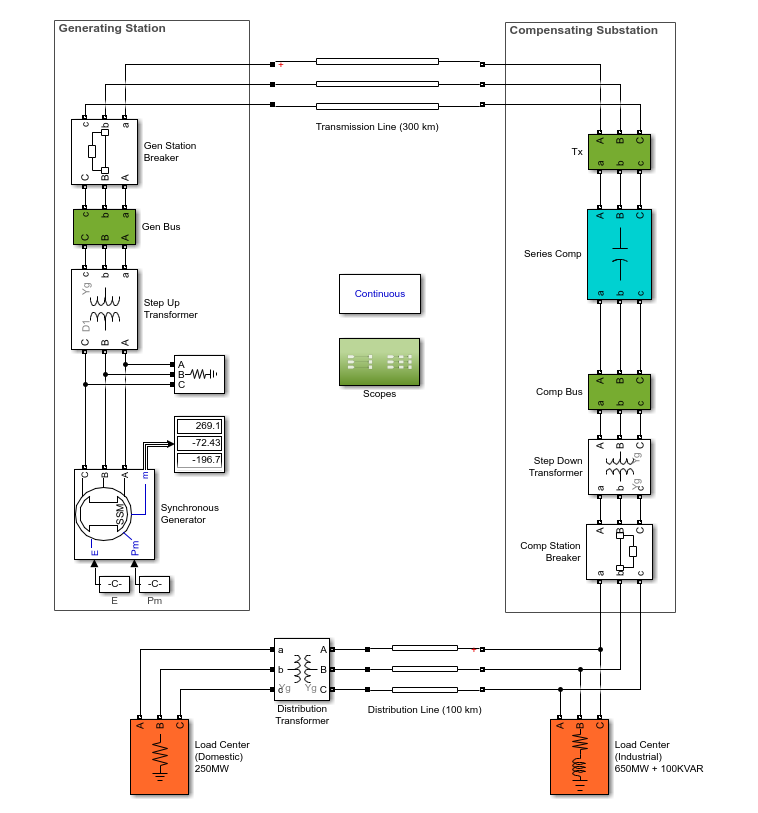
\includegraphics[width=6in]{img/model.png}
    \caption{Series Compensated Transmission Line Model}
    \label{model}
  \end{figure}

  \pagebreak
  \section{Observations}  
  \begin{figure}[H]
    \centering
    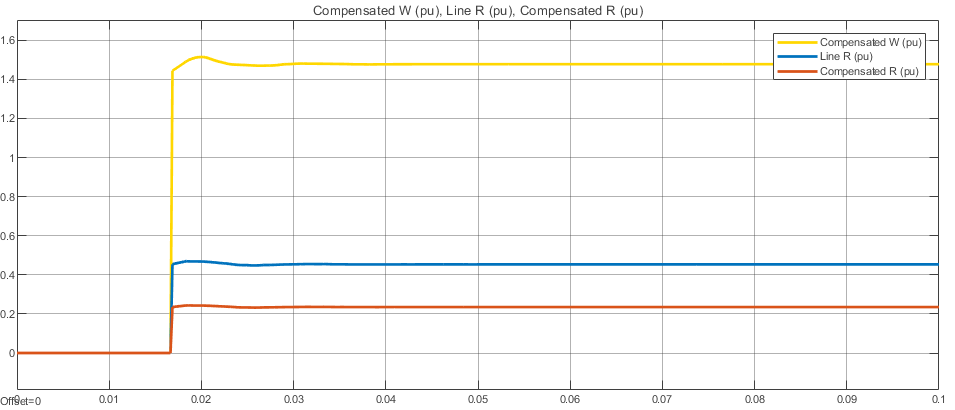
\includegraphics[width=6in]{img/compennsated.png}
    \caption{Compensation of Reactive Power}
    \label{compennsated}
  \end{figure}

  From the graph of active and reactive power we can see that the reactive power demand on the line
  was compensated by the series capacitor in the compensating substation. This reduces the load on the 
  line and thus more active power can be transmitted without needing to change the installed equipment.

  \section{Result}
  We developed a Simulink model for a series compensated transmission line, and obeserved the drop
  in reactive power demand on the line by the series capacitor in the compensating substation.

\end{document}